% !TeX root = ../main.tex
\begin{figure}[htbp]
    \centering
    \begin{subfigure}[t]{0.32\linewidth}
        \centering
        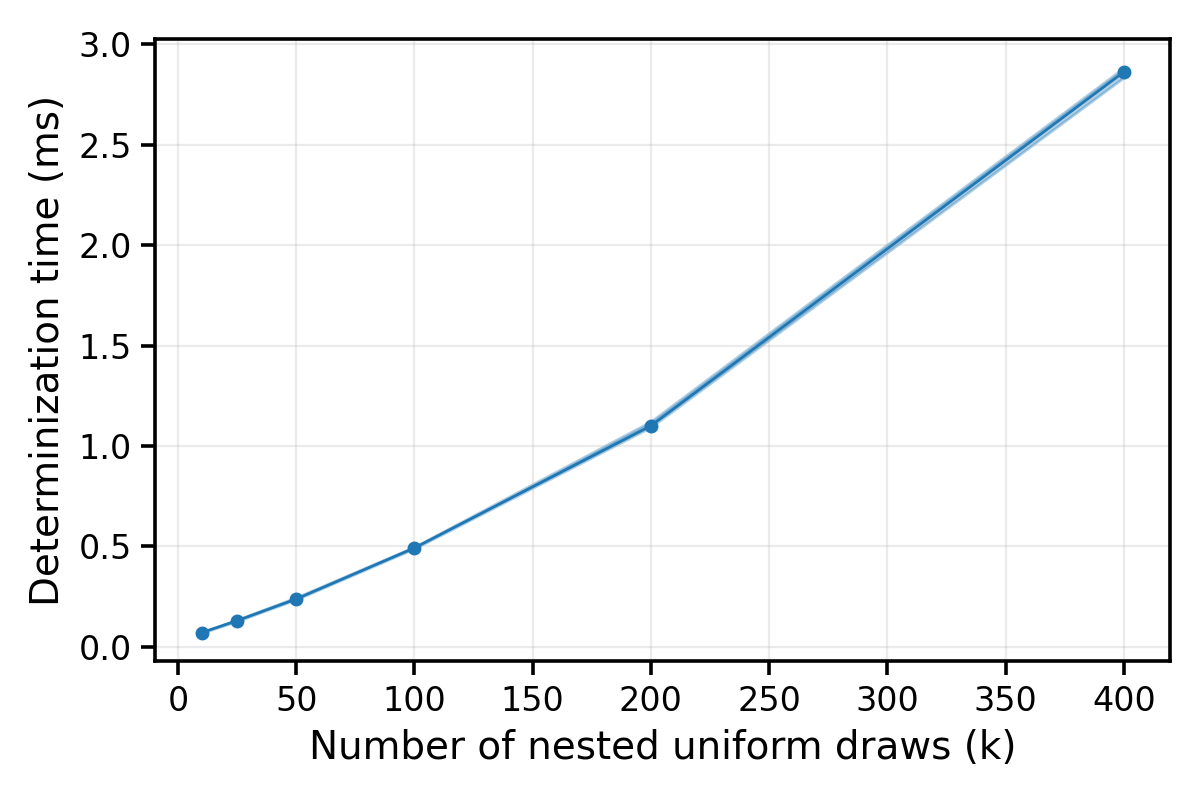
\includegraphics[width=\linewidth]{../results/scaling/uniform-nested.png}
        \caption{\texttt{uniform-nested}}
        \label{fig:scaling-uniform-nested}
    \end{subfigure}\hfill
    \begin{subfigure}[t]{0.32\linewidth}
        \centering
        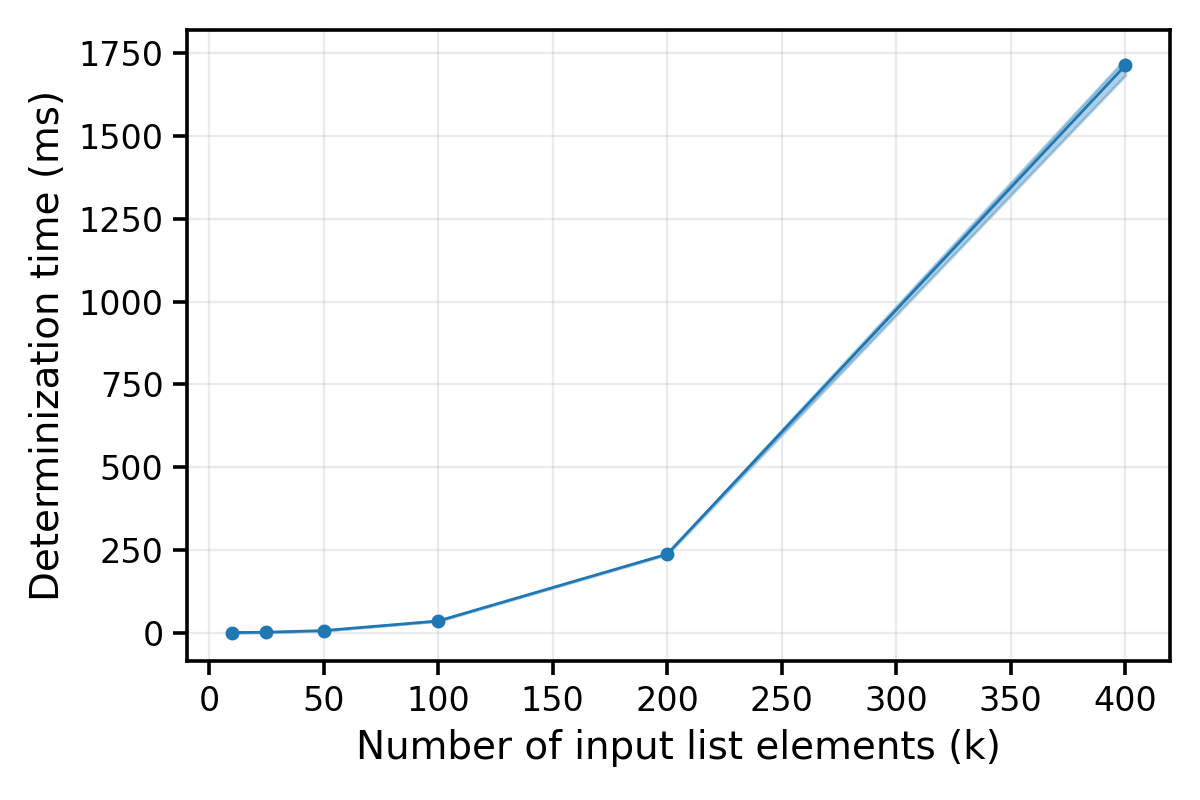
\includegraphics[width=\linewidth]{../results/scaling/gauss-random-walk.png}
        \caption{\texttt{gauss-random-walk}}
        \label{fig:scaling-gauss-random-walk}
    \end{subfigure}\hfill
    \begin{subfigure}[t]{0.32\linewidth}
        \centering
        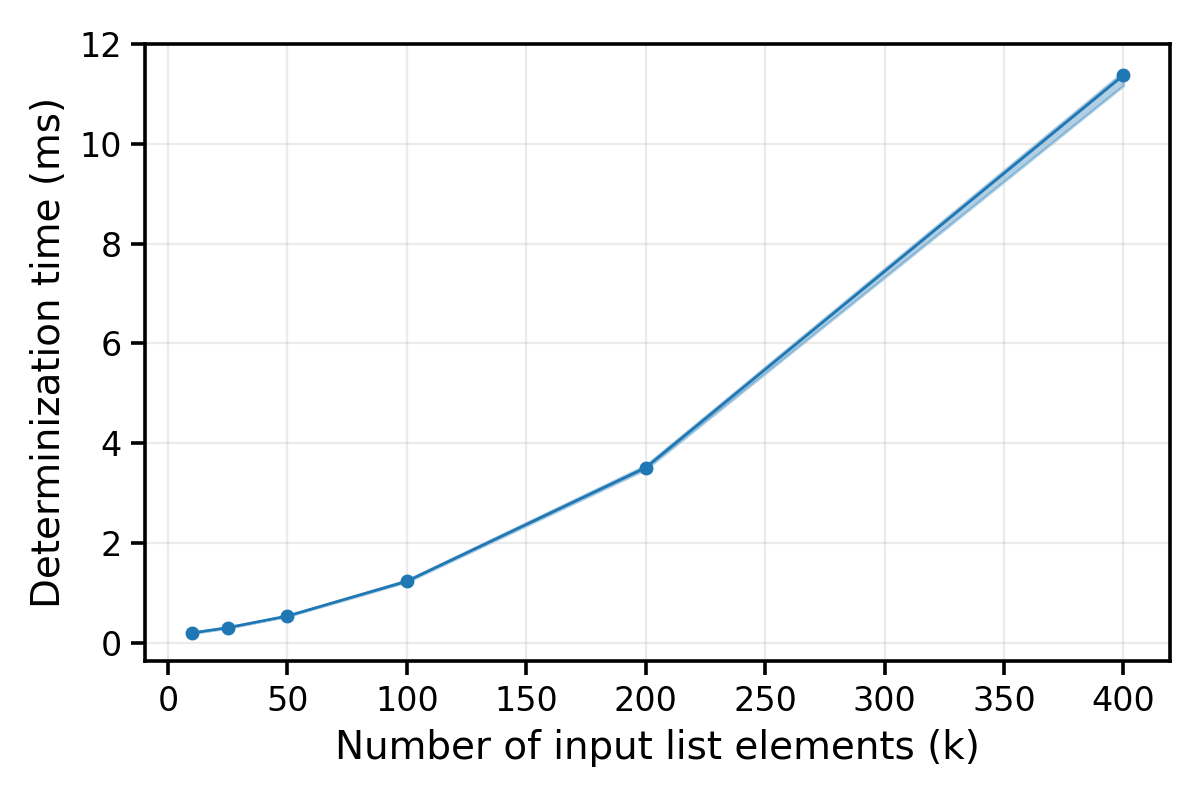
\includegraphics[width=\linewidth]{../results/scaling/add-noise.png}
        \caption{\texttt{add-noise}}
        \label{fig:scaling-add-noise}
    \end{subfigure}
    \caption{Determinization time versus the size parameter $k$. Points show median times over 10 runs;
    shaded bands show the interquartile range. Timings include determinization only.}
    \label{fig:determinization-scaling}
    \Description{Three plots show determinization time in milliseconds as the
    number of nested uniform draws increases in uniform-nested and the input-list
    length increases in the Gaussian random walk and add-noise benchmarks. Each plot includes an interquartile band.}
\end{figure}
